\documentclass[a4paper]{article}
\usepackage[utf8]{inputenc}
\usepackage{fullpage}
\usepackage[ngerman]{babel}
\usepackage{biblatex}
\bibliography{expose.bib}
\usepackage{graphicx}
\usepackage{subfigure}
\title{Augmented Reality Simulator für Sehstörungen}
\author{Willi Schönborn}
\date{\today}
\begin{document}
\maketitle

\section*{Einleitung}
Als Teil der Lehrveranstaltung \textit{Multimediatechnik Vertiefung} an der \textit{Beuth Hochschule für Technik Berlin} soll im Rahmen einer Semesterarbeit ein Projekt mit Bezügen zu den Bereichen Multimedia und Wahrnehmung entstehen. Das Ziel dieses Dokumentes ist es, die Ideen und Konzepte für dieses Projekt vorzustellen.

\begin{figure}[htbp]
\centering
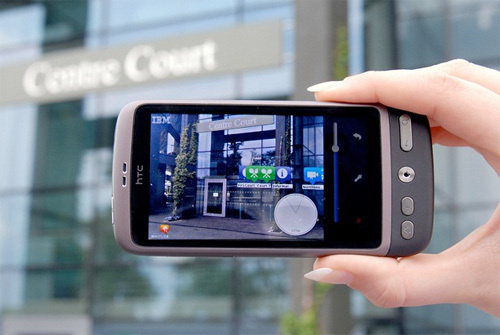
\includegraphics[width=0.45\textwidth]{500x_ibm-seer.jpg}
\caption{Augmented Reality}
\end{figure}

\section*{Idee}

Die Idee ist es, eine Android-Applikation zu entwickeln, die mithilfe der Handy-Kamera einen virtuellen Blick auf die Welt erlaubt und dabei diverse Sehstörungen simulieren kann. Das Design sowie die Benutzerschnittstelle sollten dabei so minimal wie möglich gehalten werden. Der gesamte Bildschirm stellt das aktuelle Bild der Kamera da, natürlich entsprechend modifiziert, je nach gewählter Sehstörung. Die verschiedenen Simulationen könnten beispielsweise einfach durch das Kontextmenü auswählbar sein. Mögliche Kandidaten für die Sehstörungen, die simuliert werden können sind Rot-Grün-Sehschwäche, Gelb-Blau-Sehschwäche sowie Kurzsichtigkeit. 

\begin{figure}[ht]
\centering
\subfigure[Normalsichtigkeit]{
    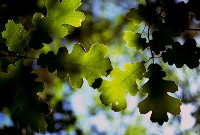
\includegraphics[width=0.3\textwidth]{leaves.jpg}
}
\subfigure[Rot-Grün-Schwäche]{
    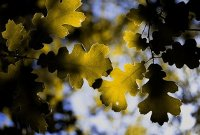
\includegraphics[width=0.3\textwidth]{leavessim.jpg}
}
\caption{Vergleich}
\end{figure}

\newpage

\nocite{gizmodo}
\nocite{android}
\nocite{wp-rotgruen}
\nocite{vischeck}
\nocite{ichbinfarbenblind}
\nocite{kurzsichtig}
\printbibliography

\listoffigures

\end{document}

